\section{Diskrete Fouriertransformation mit ANN\label{ml:dft-with-ann}}
\rhead{DFT mit ANN}

Die \emph{diskrete Fouriertransformation} (DFT) einer Zahlenreihe $x_n \in \{ x_0, x_1, \cdots, x_{N-1}\}$
mit $N$ Elementen kann mit
\begin{equation}
    c_k = \frac{1}{N} \sum_{n=0}^{N-1} x_n e^{\normalsize -jk\frac{2\pi}{N}n}
\end{equation}
berechnet werden, oder in vektorschreibweise
    \begin{equation}
    c_k = \begin{pmatrix}
        x_0\\
        x_1\\
        \vdots\\
        x_{N-1}
    \end{pmatrix} \cdot
    \frac{1}{N} \begin{pmatrix}
        e^{-j \omega_k 0} \\
        e^{-j \omega_k 1} \\
        \vdots \\
        e^{-j \omega_k (N-1)} \\
    \end{pmatrix}
    \qquad \textsf{mit}\qquad \omega_k = \frac{2\pi k}{N}.
    \label{ml:dft-with-ann:dft:vector}
\end{equation}

Die einzelnen $x_n$ werden mit einem komplexen Koeffizienten gewichtet und anschliessend
summiert. In der Vektorschreibweise wird dieser Effekt mit dem Skalarprodukt erzielt. Man
erkennt, dass dies ein linearer Zusammenhang ist. Um uns auf die reellen Zahlen zu
bschränken, wird \eqref{ml:dft-with-ann:dft:vector} in die Kosinus-Anteile $a_k = 2{\rm
Re}(c_k)$ und Sinus-Anteile $b_k = -2{\rm Im}(c_k)$ unterteilt:
\begin{equation}
    a_k = \vec x \cdot \frac{2}{N} \begin{pmatrix}
        1\\
        \cos(\omega_k 1)\\
        \vdots\\
        \cos(\omega_k (N-1))
    \end{pmatrix}
    = \vec x \cdot \vec \theta_{k,a}
    \quad \text{und} \quad
    b_k = \vec x \cdot \frac{-2}{N} \begin{pmatrix}
        0\\
        \sin(\omega_k 1)\\            
        \vdots\\
        \sin(\omega_k (N-1))
    \end{pmatrix}
    = \vec x \cdot \vec \theta_{k,b}.
\end{equation}
Beide Teile sind bis auf die Koeffizienten genau gleich. Sie können  in der Form des mehrdimensionalen linearen
Modells \eqref{ml:ann:linear-unit} als
\begin{equation}
    \vec a = \begin{pmatrix}a_0\\ \vdots \\ a_{N-1} \end{pmatrix} = \begin{pmatrix}
        \vec \theta_{0,a} & \vec \theta_{1,a} & \cdots & \vec \theta_{N-1,a}
    \end{pmatrix} \vec x
    = {\bm \thetaup}_{a} \vec x
    \quad\text{und}\quad
    \vec b = {\bm \thetaup}_{b} \vec x
\end{equation}
geschrieben werden. Die konstanten Anteile entfallen.

In Abb. \ref{fig:ml:dft-with-ann:linear} ist das Netz für die Kosinus-Anteile abgebildet.
Die Übertragungsfunktion ist somit die Identitätsfunktion $f(x) = x$. Das Netz ist
komplett linear und nicht einmal affin (alle Bias-Werte sind Null).

\begin{figure}
    \centering
    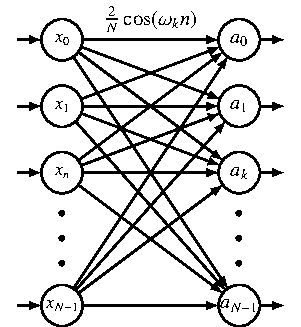
\includegraphics[scale=0.8]{papers/ml/images/ann_dft_linear.pdf}
    \caption{Lineares Netzwerk für die DFT.}
    \label{fig:ml:dft-with-ann:linear}
\end{figure}

